% Review
\documentclass[authoryear,preprint,review,12pt]{elsarticle}
%\documentclass[final,authoryear,5p,times,twocolumn,11pt]{elsarticle}

% Review topics:

% % TERMINOLOGY
% % fluid saturations or phase saturations?
% % Block-Oil, Black-oil or black-oil?


%% for a journal layout:
%% \documentclass[final,authoryear,1p,times]{elsarticle}
%% \documentclass[final,authoryear,1p,times,twocolumn]{elsarticle}
%% \documentclass[final,authoryear,3p,times]{elsarticle}
%% \documentclass[final,authoryear,3p,times,twocolumn]{elsarticle}
%% \documentclass[final,authoryear,5p,times]{elsarticle}

% Pending modifications:
% - Add bubble-point pressure to equations after volume and time integration.
% - A different fluid distribution DOES NOT lead to a different value of averaged saturation.
% - CORRECTION: saturations need not be constant in order to Bubble-point pressure be constant.

%\documentclass[final,authoryear,5p,times,twocolumn,11pt]{elsarticle}

\usepackage{lineno}
\usepackage{amsmath}
\usepackage{natbib}
\usepackage{booktabs}
%opening

\newtheorem{prop}{Proposition}
\newtheorem{remark}{Remark}
\newtheorem{step}{Step}


\begin{document}
\begin{frontmatter}
\title{Solution of thermodynamic equilibrium in black-oil reservoirs: the classical material balance equations}
%\title{Obtaining the classical material balance equations from black-oil equations}
%\journal{Journal of Petroleum Science and Engineering}
%\author{R.B. Piccinini}\ead{rbpiccinini@gmail.com}
%\address{Petrobras - UO-BA/ATP-N/RES. Salvador, Bahia, Brazil.}


\begin{abstract}
This work presents a derivation of the classical material balance equations starting from black-oil equations in integral form. The existing link between both approaches is discussed and an interpretation for pressure in material balance calculations is provided. It is shown that a condition stronger than hydrostatic equilibrium is needed to reduce black-oil equations to the classical approach. The classical equations are formulated for a variable bubble-point pressure, extending their applicability to reservoirs under pressure maintenance. Sufficient conditions for solution uniqueness are presented and a scheme for numerical solution is proposed.
\end{abstract}

\begin{keyword}
material balance \sep black-oil equations \sep reservoir engineering.
\end{keyword}
\end{frontmatter}

\section{Introduction}
The so called material balance equations are widely employed in reservoir engineering and have become a classical tool in oil reservoir management. The equations were originally presented in \cite{schilthuis1936active} and conceived as a zero dimensional model for estimating reservoir pressure from a balance of fluid production and injection. \cite{schilthuis1936active} introduced the hypothesis of thermodynamic equilibrium occurring not in the entire reservoir volume, but in the regions of high permeability where most of the produced volume would come from and where pressure would present a similar behavior. Such regions were said to contain an \textit{active oil}.

The equations developed by \cite{schilthuis1936active} did not account for the non-existence of mechanical, phase or thermal equilibrium. Also, the zero-dimensional approach excluded the possibility of mechanical equilibrium under gravity and capillary forces, which produces a variable fluid distribution in space. An attempt to introduce non-equilibrium effects of hydrodynamic origin came with \textit{black-oil} equations \citep{aziz1979petroleum,blackoil}. The novelty on hydrodynamics was the introduction of a macroscopic equation of motion employing Darcy's law.

Black-oil equations arise from the generalization of the zero dimensional concept to a multidimensional macroscopic model which incorporates hydrodynamics via Darcy's law and entails exactly the same thermodynamic approach for phase equilibrium \citep{aziz1979petroleum}.

%Although many applications of material balance equations have been reported, few explore their connection.

The term black-oil refers to specific hydrocarbon compositions whose phase equilibrium for isothermal changes in pressure may be well described by a two pseudo-component system. For such reservoir fluids, gas and oil compositions remain essentially constant in the entire range of pressure observed during reservoir productive life. 

%A general restriction of this approach is that reservoir temperature must be sufficiently below the mixture critical temperature so that different fluid phases have clearly distinguishable properties \citep{danesh1998pvt,firoozabadi1999thermodynamics}.

Since black-oil and material balance equations differ only on spatial scale and the existence of local pressure gradients, there must exist conditions under which material balance equations might be recovered from the black-oil approach. This work examines such conditions. 

This existing link was briefly addressed in \cite{ertekin2001basic}, where both approaches were argued to be equivalent if capillarity and gradients of flow potential $\Phi$ could be neglected, i.e.:
\begin{subequations}
\begin{equation}
p_\alpha = p \, ,
\end{equation}
\begin{equation}
\nabla \Phi_\alpha = \nabla p_\alpha - \rho_\alpha g \nabla z = 0 \, ,
\end{equation}
\end{subequations}
for $\alpha=o,g,w$ referring to oil, gas and water phases.

%It is shown in this work that a stronger assumption is actually needed: mechanical equilibrium in the presence of gravity ($\nabla p = \rho g \nabla z$) is not a sufficient condition, pressure gradients must identically vanish instead ($\nabla p_\alpha \equiv 0$).
%\begin{equation}
%\nabla p \equiv 0 \, .
%\end{equation}

%The restriction of a spatially constant pressure throughout the reservoir does not require PVT properties to be averaged during the integration procedure. Such averaging process is not straightforward, if not impractical, as it is shown later. For the same reason, bubble-point pressure must also be constant and it is shown that this latter assumption is equivalent to having constant fluid saturations in space.

%The requirement of a spatially constant pressure makes the material balance equations more suitable for shallow reservoirs, where gravity field is less important in phase equilibrium.

The present derivation of material balance equations allows bubble-point pressure to vary with time accordingly to the same concept widely employed in reservoir simulation, which is found in \cite{aziz1979petroleum} and \cite{ertekin2001basic}. The employed approach extends material balance equations to saturated reservoirs under pressure maintenance (e.g. fluid injection). The applicability, however, depend on how important non-equilibrium effects are to the phase equilibrium.

%It has already been shown the importance of not having strong flow near interface that prevents mixing and causes pressure to drop locally \citep{steffensen1973reservoir,utseth1981numerical}.

After presenting material balance equations, sufficient conditions for solution uniqueness are imposed on PVT properties. These conditions require fluids to be compressible and that gas dissolution occurs with reduction of the overall system volume.

A simple scheme for numerical solution is also proposed based on classical root-finding algorithms for non-linear equations.

%\section{Black-Oil Equations}
%
%Here it is used a thermodynamic fluid model known as Black-Oil \cite{blackoil}. It consists of a simplified treatment of hydrocarbon composition and phase equilibrium. Hydrocarbon species are grouped into two pseudo-components called oil and gas, being a pseudo-component one which consists of more than one chemical molecule.
%
%Oil is composed by hydrocarbon species that remain in liquid phase for standard surface pressure and temperature. The other hydrocarbon species in gaseous phase for the same surface conditions are called gas.
%
%The mixture of reservoir fluid is then composed of oil, gas and water components and can present three fluid phases: oil, gas and water. Oil phase may be composed of oil and gas components, gaseous phase may be composed uniquely by gas component and water phase uniquely by water component.
%
%In addition to the three fluid components and phases, there is a solid phase composed by the rock.
%
%The fluid phases may be defined in a more general framework so as to account for dissolution of gas in water or water vapour, for instance. Such possibilities are not dealt with in this work.
%
%For some volume containing one of the three fluid phases, the saturation of the fluid phase $k$ is defined as
%\begin{equation}\label{eq: saturation}
%S_{k}=\frac{\phi_k}{\sum_{i \neq solid} \phi_i} \, ,
%\end{equation}
%where $\phi_i$ is the volume fraction of the fluid phase $i$.
%
%In order to apply the volume balance, a control volume ($\Omega$) is defined containing all the hydrocarbon zone. It consists of the region where hydrocarbon saturation is greater than zero for some arbitrarily small volume. This reservoir definition excludes the pure water zone, which is referred to as the aquifer.
%
%
%Right hand side of Equation \eqref{eq: matbal1}, \textit{rock and fluid expansion}, is a function of phase mass transfers and compressibilities. Both should be obtained from a thermodynamic model accounting for mass transfer among phases and the relation between phase volumes and pressure. Temperature is seldom considered to vary during reservoir production and it is held constant and equal in all phases, not being an independent property of the control volume state.
%
%Such thermodynamic model is presented in detail in \cite{blackoil} and it is commonly referred to as Black-Oil Equations. The main assumption behind them is that phase and pressure equilibria are instantaneously achieved inside the control volume, i.e., mass transfer among phases reaches equilibrium and internal forces equilibrate external ones fast enough in comparison to the interval of time between two observations of control volume properties.
%
%Pressure in each phase may differ if capillary forces are taken into account, for what extra constitutive equations relating each phase pressures would be needed.
%Capillary pressure would be function of porous medium properties given by some porous medium model, e.g., permeability and porosity; phase properties, e.g., surface tension and wettability, and the thermodynamic state.
%
%Capillary pressure is very often assumed to be function of phase saturations only and, hence, the thermodynamic state of the control volume would be completely determined by the pressure of one phase (e.g. the wetting phase) and phase saturations.
%
%Black-Oil Equations do not assume water and oil phases becoming miscible for any thermodynamic state.
%
%Capillary pressure dependence on phase saturation only is often considered as a weak assumption in contradiction with experimental observations. The hysteresis of capillary pressure exhibited when either imbibition or drainage occurs is not theoretically explained and it is accounted for by empirical relations or it is rather simply neglected.
%
%\cite{hilfer1} has proposed the inclusion of an energy equation.

\section{Derivation of equations}

This section starts presenting black-oil equations and it proceeds averaging quantities in space and examining simplifying assumptions for wich material balance equations are obtained.

\subsection{Black-Oil equations}

As already mentioned, black-oil is a designation to a simplified treatment of hydrocarbon composition and phase equilibrium. Hydrocarbon species are grouped into two pseudo-components called oil and gas, being a pseudo-component one that consists of more than one chemical molecule.

Oil component, also called stock tank oil, is defined as the hydrocarbon composition in liquid phase for standard surface pressure and temperature. Similarly, gas component is the hydrocarbon composition in gaseous phase for the same surface conditions. All species are generally present in both phases although the equilibrium composition is shifted to liquid phase (or gaseous phase) for components of greater (lower) molecular mass.

Reservoir fluids are then composed of the two pseudo-components (oil and gas) plus the water component. There can exist three fluid phases: oil, gas and liquid water. Oil phase may be composed of oil and gas components, gas phase may be composed uniquely by the gas component and, water phase, uniquely by water component. The only allowed mass transfer is of gas component between oil and gas phases.

In addition to the three fluid components and phases, there is the solid phase composed by the rock.

Mass balance equations for each component in fluid phase are:

\begin{itemize}
\item water component:
\begin{equation}\label{eq: Sw1}
\frac{\partial}{\partial t} \int\limits_{\Omega} \rho_w S_w \phi dV + \oint_{\partial \Omega} \rho_w \left( \mathbf{u}_w \cdot \mathbf{dS} \right) = \rho_w^{ST}Q_w^{ST} \, ;
\end{equation}

\item oil component:
\begin{equation}\label{eq: So1}
\frac{\partial}{\partial t} \int\limits_{\Omega} \rho_o Y_o S_o \phi dV + \oint_{\partial \Omega} \rho_o Y_o \left(\mathbf{u}_o \cdot \mathbf{dS} \right)= \rho_o^{ST}Q_o^{ST} \, ;
\end{equation}

\item gas component:
\begin{equation}\label{eq: Sg1}
\frac{\partial}{\partial t} \int\limits_{\Omega} \left( \rho_o Y_g S_o + \rho_g S_g\right) \phi dV + \oint_{\partial \Omega} \left( \rho_o Y_g \mathbf{u}_o + \rho_g \mathbf{u}_g\right) \cdot \mathbf{dS}= \rho_g^{ST}Q_g^{ST} \, .
\end{equation}
\end{itemize}
Mass concentration of oil and gas components in oil phases are denoted as $Y_o$ and $Y_g$, respectively.

Phase saturation is defined as its volumetric fraction of the pore space:
\begin{equation}
S_\alpha = \frac{\phi_\alpha}{\phi} \, ,
\end{equation}
where $\phi_\alpha$ is the volumetric fraction of a fluid phase $\alpha$ and $\phi$ is the porosity, i.e., the volumetric fraction of the pore volume. Since we consider that pore volume is fully saturated with fluid,
\begin{equation}
S_o + S_g +S_w = 1 \, .
\end{equation}

A common simplification in black-oil formulations is to restrict mass transport to macroscopic advection. No diffusive or dispersive term is included in the mass balance equations. This simplification must be looked with care when gradients of species concentration are important and $\nabla Y_i \approx 0$ does not hold for some species $i$. For instance, when gas is being dissolved in oil phase in a reservoir under repressurization, this condition is not generally true.

%Mass balance equations for each fluid phase are \citep{ertekin2001basic}:
%% Oleo
%\begin{equation}\label{eq: So1}
%\frac{\partial}{\partial t}\left(\frac{\phi(p_P) S_o}{B_o(p_o,P_b)}\right)+\nabla\cdot\left(\frac{\mathbf{u}_o}{B_o (p_o,P_b)}\right)=q_{os} \, ,
%\end{equation}
%% Gas
%\begin{equation}
%\begin{split}\label{eq: Sg1}
%\frac{\partial}{\partial t}\left[\phi(p_P)\left(\frac{S_g}{B_g (p_g)} +\frac{S_o R_s (p_o,P_b)}{B_o (p_o,P_b)}\right)\right] \\
%+\nabla\cdot\left(\frac{\mathbf{u}_o R_s (p_o,P_b)}{B_o (p_o,P_b)}+\frac{\mathbf{u}_g}{B_g (p_g)}\right)=q_{gs} \, ,
%\end{split}
%\end{equation}
%% Agua
%\begin{equation}\label{eq: Sw1}
%\frac{\partial}{\partial t}\left(\frac{\phi (p_P) S_w}{B_w (p_w)}\right)+\nabla\cdot\left(\frac{\mathbf{u}_w}{B_w(p_w)}\right)=q_{ws} \, ,
%\end{equation}
%
%where saturations must satisfy the constraint
%\begin{equation}\label{eq: S11}
%S_o+S_w+S_g=1 \, .
%\end{equation}
%
%Bubble-point pressure ($P_b$) is here defined as the minimum pressure for which gas phase is locally absent, i.e., $S_g=0$. Its local value is implicitly given by the solubility ratio ($R_s$) satisfying the equation:
%\begin{equation}\label{eq: Pb}
%R_s(p_o=P_b,P_b) = \frac{B_g(p_g)}{B_o(p_o,P_b)}\frac{S_g}{S_o} +R_s(p_o,P_b) \, .
%\end{equation}
%It must be remarked that bubble-point pressure is sometimes defined in a different manner as the bubble-point pressure for the hydrocarbon composition in oil phase only. According to this latter definition, $P_b = p_o$ for any saturated reservoir.
%
%Black-oil equations make the assumption of instantaneous mass transfer between oil and gas phases, what is only reasonable for a reservoir under depletion, when oil and gas components are homonegeously distributed in oil phase. Once constant temperature and fluid composition are assumed, diffusion and advection of species and energy become unimportante for phase equilibrium calculations.
%
%If gradients of species concentration are present within oil phase, however, as it occurs in saturated reservoirs under pressure maintenance, a combined mechanism of advection and diffusion exists and those are absent of black-oil equations. Some heuristic models have been proposed for problems where this issue is critical, as for gas injection projects. \cite{utseth1981numerical} has proposed to limit $dR_s/dt$ and neglect transport of gas component in oil phase for a simplified treatment.

Momentum balance for each phase is given by an extension of Darcy's law to multiphase flow. This extension consists in multiplying absolute (or single-phase) permeability ($\mathbf{k}$) by a scalar function called phase relative permeability ($k_{r,\alpha}$):

\begin{equation}\label{eq: exdarcy}
\mathbf{u}_\alpha = -\frac{k_{r,\alpha} \mathbf{k}}{\mu_\alpha} \left(\nabla p_\alpha - \rho_\alpha g\nabla z\right) \, , \quad \alpha=o,w,g \, .
\end{equation}

Phase densities are functions of the local thermodynamic state:
\begin{equation}
\rho_w = \rho_w \left(p_w, T_w\right)
\end{equation}
\begin{equation}
\rho_o = \rho_o \left(p_o, T_o,Y_g\right)
\end{equation}
\begin{equation}
\rho_g = \rho_g \left(p_g, T_g\right)
\end{equation}

Another simplification is now made assuming thermal equilibrium in the entire reservoir volume:
\begin{equation}
T_w = T_o = T_g = T
\end{equation}
and
\begin{equation}
\nabla T \equiv 0 \, .
\end{equation}

Temperature is thus a constant prescribed value and no energy balance equation is needed. Also, it follows from Gibbs' phase rule that the equilibrium of oil and gas phases has only two degrees of freedom if we restrict component number to the two pseudo-components. As temperature is assumed constant, oil phase density in saturated states is a function of pressure or composition only. The same is valid for mass concentrations of gas and oil components in oil phase.

\begin{equation}
Y_g = Y_g (p) \, ,
\end{equation}
\begin{equation}
Y_o = Y_o (p) \, .
\end{equation}

Porosity ($\phi$) is assumed a function of pore pressure ($p_P$). Since three phases are present in general, such quantity is defined by some relation of type \citep{kim2011rigorous}:
\begin{equation}
p_P=p_P\left(p_o,p_w,p_g,S_o,S_w,S_g\right) \, .
\end{equation}

In order to close the system of equations, a connection among different phase pressures must be provided. Such expressions are referred to as capillary pressures and are usually employed in the following forms \citep{aziz1979petroleum}:
%capillary
\begin{equation}\label{eq: capillary_ow}
p_{c,ow}\left(\mathbf{k},\phi,S_w\right)=p_o-p_w \, ,
\end{equation}
\begin{equation}\label{eq: capillary_og}
p_{c,go}\left(\mathbf{k},\phi,S_g\right)=p_g-p_o \, .
\end{equation}


%Capillary pressure and relative permeability are controversial concepts in the sense that they have not been demonstrated to arise from theoretical foundations. For practical applications, both functions are usually assumed in the forms presented above and their properties are argued to be empirically established.

%It is well known that black-oil equations possess discontinuous solutions in saturation, bubble pressure and solubility ratio fields. Discontinuities (or shocks) are introduced by initial or boundary conditions and are propagated throughout flow domain due to the hyperbolicity of equations.
%
%In initial conditions, if hydrostatic equilibrium is imposed and no capillary pressure is included, that is,
%\begin{equation}
%p_{c,ow}=p_{c,og}=0 \quad \longrightarrow \quad p_o=p_w=p_g=p\, ,
%\end{equation}
%saturation discontinuities will be present due to gravity segregation.
%
%When capillary pressure is present and it is function of phase saturations, a diffusive term is introduced in mass balance equations and shocks originated by phase displacement become smoothed:
%\begin{equation}
%\frac{\partial}{\partial t}\left(\frac{\phi (p_P) S_w}{B_w (p_w)}\right)-\nabla\cdot\left[\frac{k_{r,w} \mathbf{k}}{B_w(p_w)\mu_w} \left(\nabla p_o - \rho_w g\nabla z -\underbrace{\frac{d p_c}{d S_w}\nabla S_w}_{\text{water diffusion}}\right)\right]=q_{ws} \, .
%\end{equation}
%
%Discontinuities in saturation may still occur, however, if capillary pressures are functions of discontinuous porous medium properties ($phi$ and $\mathbf{k}$) or if phase change takes place, as diffusion of gas dissolved in oil phase is not allowed.
%Cite Bear and Herrera.


\subsection{Material balance equations}

Derivation of the classical material balance equations consists in assuming no fluid motion and in integrating black-oil equations in the entire reservoir volume. The integration process, however, requires all quantities to be either averaged or assumed constant in space.

%Defining averages of most quantities is difficulty, though, as they appear in equations as products of up to three factors. Being the quantities self-correlated, the averaging process would involve unclosed terms. Quantities are thus required to be spatially constant wherever needed.

%A second problem is that averaging requires the knowledge of a spatial distribution of quantities for it be uniquely specified, as it can be seen for an average saturation depending on spatial distributions of local saturation and porosity,
%\begin{equation}\label{eq: avS}
%\bar{S}_\alpha = \int_\Omega S_\alpha \phi dV \, .
%\end{equation}


We start assuming mechanical equilibrium, i.e., no bulk motion:
\begin{equation}
\mathbf{u}_\alpha = -\frac{k_{r,\alpha} \mathbf{k}}{\mu_\alpha} \left(\nabla p_\alpha - \rho_\alpha g\nabla z\right)\equiv 0 \, .
\end{equation}
This condition implies that pressure gradients must equal gravity force per unit volume:
\begin{equation}\label{eq: p=rhogh}
\nabla p_\alpha = \rho_\alpha g\nabla z
\end{equation}
and, consequently, pressure is a function of depth only:
\begin{equation}\label{eq: p=rhogh}
\int_{p_\alpha^0}^{p_\alpha} \frac{dp_\alpha^{'}}{\rho_\alpha \left(p_\alpha^{'},T\right)} = g\left(z - z_0\right) \, .
\end{equation}

Black-oil equations then become:
\begin{itemize}
\item water component:
\begin{equation}\label{eq: Sw2}
\frac{\partial}{\partial t} \int\limits_{\Omega} \rho_w S_w \phi dV = \rho_w^{ST}Q_w^{ST} \, ;
\end{equation}

\item oil component:
\begin{equation}\label{eq: So2}
\frac{\partial}{\partial t} \int\limits_{\Omega} \rho_o Y_o S_o \phi dV = \rho_o^{ST}Q_o^{ST} \, ;
\end{equation}

\item gas component:
\begin{equation}\label{eq: Sg2}
\frac{\partial}{\partial t} \int\limits_{\Omega} \left( \rho_o Y_g S_o + \rho_g S_g\right) \phi dV = \rho_g^{ST}Q_g^{ST} \, .
\end{equation}
\end{itemize}
%
\subsubsection{Averaging quantities}

We now define space averaged quantities for porosity ($\phi$), saturation ($S_\alpha$) and density ($\rho_\alpha$) of a phase $\alpha$ and mass concentration of a component $k$ in phase $\alpha$ ($Y_{\alpha,k}$).

All quantities are locally functions of space and time, but, after averaged in space, they become functions of time only:

\begin{equation}
\bar{\phi} (t) = \frac{1}{\Omega}\int_{\Omega}\phi \left(\mathbf{x},t\right) dV \, .
\end{equation}

We proceed omitting function arguments:
\begin{equation}
\bar{S_\alpha}\bar{\phi} = \frac{1}{\Omega}\int_{\Omega}S_\alpha \phi dV \, ,
\end{equation}

\begin{equation}
\bar{\rho_\alpha}\bar{S_\alpha}\bar{\phi} = \frac{1}{\Omega}\int_{\Omega}\rho_\alpha S_\alpha \phi dV \, ,
\end{equation}

\begin{equation}
\bar{\rho_\alpha}\bar{Y_{\alpha,k}}\bar{S_\alpha}\bar{\phi} = \frac{1}{\Omega}\int_{\Omega}\rho_\alpha Y_{\alpha,k} S_\alpha \phi dV \, .
\end{equation}

Eqs. \eqref{eq: Sw2}, \eqref{eq: So2} and \eqref{eq: Sg2} rewritten in terms of averages read:

\begin{itemize}
\item water component:
\begin{equation}\label{eq: Sw3}
\frac{\partial}{\partial t} \left( \bar{\rho_w}\bar{S_w}\bar{\phi} \Omega \right) = \rho_w^{ST}Q_w^{ST}
\end{equation}

\item oil component:
\begin{equation}\label{eq: So3}
\frac{\partial}{\partial t} \left( \bar{\rho_o}\bar{Y_o}\bar{S_o}\bar{\phi} \Omega \right) = \rho_o^{ST}Q_o^{ST}
\end{equation}

\item gas component:
\begin{equation}\label{eq: Sg3}
\frac{\partial}{\partial t} \left[\left( \bar{\rho_o}\bar{Y_g} \bar{S_o} + \bar{\rho_g} \bar{S_g} \right) \bar{\phi} \Omega\right] = \rho_g^{ST}Q_g^{ST} \, .
\end{equation}
\end{itemize}

We shall now introduce very common definitions from petroleum engineering for the description of volumetric and solubility changes in fluid phases. In what concerns volumetric changes, $B_w$, $B_o$ and $B_g$, the formation volume factors of water, oil and gas phases, respectively, express the ratio of a phase volume at some given pressure and temperature condition to the volume of the same phase at standard pressure and temperature, i.e.:

\begin{equation}\label{eq: Bw}
B_w = \frac{\rho_w^{ST}}{\bar{\rho_w}} \, ,
\end{equation}

\begin{equation}\label{eq: Bo}
B_o = \frac{\rho_o^{ST}}{\bar{Y_o} \bar{\rho_o}} \, ,
\end{equation}

\begin{equation}\label{eq: Bg}
B_g = \frac{\rho_g^{ST}}{\bar{\rho_g}} \, .
\end{equation}

In what concerns changes in gas solubility in oil phase, the solubility ratio ($R_s$) gives the ratio between dissolved gas component volume and oil component volume both measured in standard condition:

\begin{equation}
R_s = \frac{\rho_o^{ST} / \bar{Y_o}}{\rho_g^{ST} / \bar{Y_g}} \, ,
\end{equation}

or using $\bar{Y}_o + \bar{Y}_g = 1$:
\begin{equation}
R_s = \frac{\rho_o^{ST}}{\rho_g^{ST}}\frac{\bar{Y}_g}{1-\bar{Y}_g} \, .
\end{equation}

\subsubsection{Definition of a reference depth for pressure}

Applications of material balance equations are widely employed to stablish a relation between production (and injection) and reservoir pressure. It turns out, as we know, that pressure is different for different locations, mostly for different values of depth, and also for different phases.

What is then the significance of a single value of pressure for the entire reservoir, i.e., the reservoir pressure? 

We shall see that for the purpose of computing phase densities in the material balance, if we define a reference depth and use the corresponding local pressure, no important error is introduced in computing density. Phase pressure increases with depth according to the hydrostatic gradient. The pressure increase, however, is not significant to produce appreciable variation in phase density.

%and it may be approximated to a constant density measured at some reference depth.

We may quantify this approximation by putting together the expressions for fluid compressibility and hydrostatic equilibrium.
For this, we assume a constant isothermal compressibility to oil phase
\begin{equation}\label{eq: grado}
\left( \frac{1}{\rho_o}\frac{\partial \rho_o}{\partial p_o} \right)_{T,Y_o} = c_o 
\end{equation}
and we use hydrostatic equilibrium $dp_o = \rho_o g dz$ to obtain the expression for the derivative of oil density with depth:
\begin{equation}
\left( \frac{1}{\rho_o}\frac{\partial \rho_o}{\partial z} \right)_{T,Y_o} = c_o \rho_o g \, .
\end{equation}

Similarly for the gas phase, we obtain its isothermal compressibility from the gas state equation
\begin{equation}
\left(\frac{1}{\rho_g}\frac{\partial \rho_g}{\partial p_g}\right)_{T,Z} = \frac{1}{p_g} = \frac{\mathcal{M}}{\rho_g ZRT}
\end{equation}
and again we use hydrostatic equilibrium to obtain the derivative of gas density with depth:
\begin{equation}\label{eq: gradg}
\left(\frac{1}{\rho_g}\frac{\partial \rho_g}{\partial z}\right)_{T,Z} = \left(\frac{\mathcal{M}}{ Z R T}\right) g \, .
\end{equation}


Substituting typical values in Eqs.~\eqref{eq: grado} and \eqref{eq: gradg}, we see that oil and gas densities are rather constant with depth:
\begin{equation}
\left(\frac{1}{\rho_o}\frac{\partial \rho_o}{\partial z}\right)_{T,Y_o} \approx 10^{-6}\ m^{-1} \, ,
\end{equation}

\begin{equation}
\left(\frac{1}{\rho_g}\frac{\partial \rho_g}{\partial z}\right)_{T,Z} \approx 10^{-5}\ m^{-1} \, .
\end{equation}

The reference depth for computing fluid density (or formation volume factors) is then any arbitrary depth inside phase volume. 

For the case of an oil reservoir covered by a gas cap, the reference depth may be defined with advantage at the gas-oil contact. The point is that at the contact, both gas and oil densities may be computed using the same pressure, i.e., the corresponding local value. 

If the reference depth for oil phase is otherwise defined below gas-oil contact, gas density must be computed at some different depth still inside gas phase. This is to avoid the effect of oil hydrostatic gradient in the computation of gas density,
\begin{equation}
\left(\frac{1}{\rho_g}\frac{\partial \rho_g}{\partial z}\right)_{T,Z} = \frac{\rho_o}{\rho_g}\left(\frac{\mathcal{M}}{Z R T}\right)g  \, ,
\end{equation}
what is $\rho_o / \rho_g$ times greater than the pure effect of gas hydrostatic pressure on its density.

\subsubsection{Material balance as a pressure equation}

Equations may now be rewritten using the above definitions and denoting porous volume by $V_p = \bar{\phi}\Omega$.

\begin{equation}\label{eq: Sw4}
\frac{\partial}{\partial t} \left(\frac{\bar{S_w} V_p}{B_w} \right) = Q_w^{ST} \, ,
\end{equation}

\begin{equation}\label{eq: So4}
\frac{\partial}{\partial t} \left(\frac{\bar{S_o} V_p}{B_o} \right) = Q_o^{ST} \, ,
\end{equation}

\begin{equation}\label{eq: Sg4}
\frac{\partial}{\partial t} \left[ V_p \left(\frac{\bar{S_g}}{B_g} + \frac{\bar{S_o} R_s}{B_o} \right) \right] = Q_g^{ST} \, ,
\end{equation}

\begin{equation}\label{eq: S14}
\bar{S_w}+\bar{S_o}+\bar{S_g}=1 \, .
\end{equation}

Integrating above equations between times $t_1$ and $t_2$ gives:
% Water
\begin{equation}\label{eq: Sw5}
\frac{V_{p2} \bar{S}_{w2}}{B_{w2}}=W+\left(W_i+W_e-W_p\right) \, ,
\end{equation}

% Oil
\begin{equation}\label{eq: So5}
\frac{\bar{S}_{o2} V_{p2}}{B_{o2}} = N-N_p \, ,
\end{equation}

% Gas
\begin{equation}\label{eq: Sg5}
V_{p2}\left(\frac{\bar{S}_{g2}}{B_{g2}} +\frac{\bar{S}_{o2} R_{s2}}{B_{o2}}\right) = N\left(m\frac{B_{o1}}{B_{g1}} + R_{s1}\right) +\left(G_i-G_p\right) \, ,
\end{equation}
%
\begin{equation}\label{eq: S15}
S_o+S_w+S_g=1 \, .
\end{equation}

Where $N=V_{p1} \bar{S}_{o1}/B_{o1}$ and $W=V_{p1} \bar{S}_{w1}/B_{w1}$ are the initial volumes of oil and water measured at standard conditions and $m=V_{p1} \bar{S}_{g1}/B_{o1} N$ is the ratio of the initial volumes of gas and oil measured in reservoir conditions.

An equation for bubble-point may be obtained by setting $S_g=0$ in Eq.~\eqref{eq: Sg5} and solving it for the solubility ratio at bubble-point pressure $R_s(p=P_b)$:
\begin{equation}
\begin{split}
R_{s2}\left(p=P_b\right) = &\Big[N\left(m B_{1}/B_{g1} +R_{s1}\right)\\
&+G_i-G_p\Big]/\left(N-N_p\right) \, .
\end{split}
\end{equation}

%Equations from \eqref{eq: Sw4} to \eqref{eq: S14} constitute the most general form of material balance equations. So far, the only simplification made to black-oil equations was the absence of fluid motion, allowing pressure to be computed from Eqs.\eqref{eq: capillary_ow}, \eqref{eq: capillary_og} and \eqref{eq: p=rhogh}, and equations to be integrated in the entire reservoir volume.

We now look to solve Eqs. \eqref{eq: Sw5}, \eqref{eq: So5} and \eqref{eq: Sg5} for the averaged quantities. 


A single equation for pressure may be obtained by substituting Eqs.~\eqref{eq: So2}, \eqref{eq: Sg2} and \eqref{eq: Sw2} into \eqref{eq: S12}. The resulting equation allows pressure to be calculated from given production ($F_p$) and injection ($F_i$) volumes:
\begin{equation}\label{eq: MBE}
F_p - F_i= \underbrace{N E_o + mN E_g + W E_w}_{\text{fluid volume expansion } (E)} +\underbrace{V_{p1}-V_{p2}}_{\text{porous volume contraction } (C)}
\end{equation}
or
\begin{equation}\label{eq: MBE_short}
F_p - F_i= E + C \, ,
\end{equation}

where newly introduced terms are defined in Table~\ref{tab: MBE}. Eq.~\eqref{eq: MBE} is commonly referred to as the Material Balance Equation (MBE).

\section{Solution of Material Balance Equations}
A numerical solution of Eq.~\eqref{eq: MBE_short} is presented here. We shall start defining a residual function ($\varepsilon$) for which the pressure solving Eq.~\eqref{eq: MBE_short} is a root:
\begin{equation}\label{eq: residual}
\varepsilon(p_2) = \frac{E+F_i+C-F_p}{V_{p1}} \, .
\end{equation}
We proceed showing that $\varepsilon$ is a monotonic function provided some conditions on fluid properties are observed and that, as a consequence, only one root of $\varepsilon$ exists at most. Equivalently, we may say that only one solution exists for material balance equation.

%The conditions imposed on fluid PVT properties are the mathematical equivalent of requiring a far from critical thermodynamic state.

\subsection{Mathematical Aspects of the Residual Function}

It is a known result of real analysis that a monotonic function $f:D\subset\mathcal{R}\rightarrow\mathcal{R}$ can have at most one root in $D$. Further, if $f$ is continuous in the closed interval $I=[a,b] \subset D$ and $f(a)f(b)<0$, then $f$ has one (and only one) root in $I$.

We now state without proof that the following affirmatives are sufficient conditions to classify a function $f$ as monotonic:
%We now show that $\varepsilon$ is a monotonic function since it is:
\begin{itemize}
\item $f$ is continuous;
\item $f$ is differentiable everywhere except for a countable set of points;
\item $f'<0$ everywhere.
\end{itemize}

Residual function clearly satisfies the first two affirmatives because fluid properties are continuous everywhere and are also differentiable everywhere except at bubble-point pressure.
The last affirmative is proved by rewriting $d\epsilon/dp$ as a sum of four parcels corresponding each one to a different phase. Each phase parcel is composed of two factors: current volume \textit{in-situ} and volume derivative with respect to pressure:
\begin{equation}
\begin{split}
&V_{p1}\frac{d\varepsilon}{dp}=\underbrace{\left(N-N_p\right) \left(\frac{dB_o}{dp} - B_g \frac{dR_s}{dp} \right)}_\text{oil phase}\\
&+\underbrace{\left[N R_{s1}+mN\frac{B_{o1}}{B_{g1}}+G_i-\left(N-N_p\right)R_{s2}-G_p\right] \frac{dB_g}{dp}}_\text{gas phase}\\
&+\underbrace{\left(W + W_i+W_e-W_p\right)\frac{dB_w}{dp}}_\text{water phase}\\
&\underbrace{-\frac{dV_p}{dp}}_\text{porous volume}\, .
\end{split}
\end{equation}

\textit{In-situ} volumes (e.g. $N-N_p$ for oil phase) are clearly non-negative values. Pressure derivatives of fluid volumes are all negative values (as fluid pressure increases, fluid volume contracts) and pressure derivative of rock porous volume is a positive value (as fluid pressure increases, porous volume expands).

The value of $d\varepsilon/dp$ is thus negative because each term is a product of a negative and a positive value, being the sum of all the four terms also a negative value.

In summary, the following four relations constitute sufficient conditions for $\varepsilon(p)$ be a strictly decreasing function and for material balance equations to have only one solution:
\begin{equation}\label{eq: PVTH1}
\left(\frac{dB_o}{dp} - B_g \frac{dR_s}{dp} \right) <0 \, ,
\end{equation}
\begin{equation}\label{eq: PVTH2}
\frac{dB_g}{dp} < 0 \, ,
\end{equation}
\begin{equation}\label{eq: PVTH3}
\frac{dB_w}{dp} < 0 \, ,
\end{equation}
\begin{equation}\label{eq: PVTH4}
-\frac{dV_p}{dp}<0 \, .
\end{equation}

Switching inequalities to equalities in Eqs.~\eqref{eq: PVTH1}, \eqref{eq: PVTH2} and \eqref{eq: PVTH3} is equivalent to enforcing system incompressibility. Eq.~\eqref{eq: PVTH1}, for instance, would require a volume increase in oil phase to be equal to gas volume in gas phase for any additional gas dissolution.

\subsection{Solution Algorithm}
Several methods exist to find roots of nonlinear continuous functions \citep{hamming1987numerical}. One possible choice is Newton's method, which linearizes the function using either its gradient or a secant line. The secant line approach introduces an artificial smoothness to the gradient direction near continuous but non-differentiable points, for what it is the approach employed here to deal with the bubble-point pressure.

An open source implementation of secant method is available in SciPy library \citep{scipy}. This work used library version $0.12$.

%A more simple and robust option is the bisection method, which does not require the function to be differentiable anywhere. The number of iterations $n$ required to reduce search interval by a factor of $\delta$ is \citep{hamming1987numerical}:
%\begin{equation}
%n=\log_{2} (\delta)+1 \, .
%\end{equation}

%If the inital search interval is $[a;b]$, an error tolerance $|p^{n}-p^{n-1}|\leq (b-a)/\delta $ can be achieved in $21$ iterations for $\delta=10^{6}$.

%Either methods were successfully employed to obtain solution of equations.

The steps to solve all material balance equations are summarized bellow:
\begin{step}
Compute bubble-point pressure for instant $t_2$.
\end{step}

Bubble-point pressure $P_{b2}$ is only a function of the values in initial instant $t_1$ and produced and injected volumes.

\begin{step}
Compute fluid pressure for instant $t_2$ finding the root of residual function ($\varepsilon$).
\end{step}

Pressure in Eq.~\eqref{eq: MBE} is only a function of fluid properties in instant $t_1$, produced and injected values and bubble-point pressure at instant $t_2$, $P_{b2}$, which was already computed in step 1.

\begin{step}
Compute fluid saturations $t_2$.
\end{step}

Once $S_{o2}$, $S_{g2}$, $S_{w2}$, $p_2$ and $P_{b2}$ are known, solution for instant $t_2$ is complete.

\section{Results}
Material balance equations were solved for a black-oil reservoir initially producing in depletion drive mechanism and later subjected to water injection. Fig.~\ref{fig: matbal_p} shows in the solid line curve the severe depletion during initial phases of production. In the dashed curve, Fig.~\ref{fig: matbal_p} shows the bubble-point pressure, indicating how far the saturated reservoir is from undersaturation and allowing for planning of pressure maintenance projects.


Water injection starts when oil recovery factor $(RF)$ is about $RF=0.08$ and it is maintained until the reservoir reaches a novel undersaturated state. Initially, the high compressibility of gas prevents pressure from raising and free gas phase is reduced due to redissolution. Finally, the reservoir reaches the undersaturated state and a steep pressure increase is seen in Fig.~\ref{fig: matbal_p} for a recovery factor about $RF=0.15$.

It must be observed that the result of gas reentering oil phase completely neglects non-equilibrium effects, e.g. compositional gradients, and must be used with care. For instance, it may be in strong disagreement with real reservoir behavior when gravity segregation is present.

Figure~\ref{fig: matbal_s} shows the formation of a free gas phase with growing $S_g$ and then its disappearance. Depending on the ratio of vertical and horizontal permeabilities or reservoir dip angle, it may also suggest the formation of a secondary gas cap.

Figure~\ref{fig: epsilon} shows the shape of residual function ($\epsilon$) with respect to pressure, i.e, holding all produced or injected volumes constant and allowing only pressure to change. Each different solid line corresponds to a different volume of fluid production and injection. The function root is the solution of material balance equation, Eq.~\eqref{eq: MBE_short}, and the non-differentiable point is the bubble-point pressure. Also, it is seen that function $\epsilon$ monotonically decreases with pressure, as theoretically shown before.

Figure~\ref{fig: iter} shows the count of newtonian iterations required to compute pressure with an accuracy within $0.001$ of initial bubble-point pressure. Typically, $12$ iterations are required.

Figure~\ref{fig: residual} shows the residual of numerical solution as defined in Eq.~\eqref{eq: residual}. Material balance error is bellow $10^{-7}$ units of porous volume for all time steps.



\section{Conclusions}
\begin{enumerate}[1.]
\item Material balance equations can be obtained from black-oil equations under the assumptions of:
\begin{enumerate}[(a)]
\item mechanical equilibrium;
\item absence of gravity and capillary forces;
\item spatially constant bubble-point pressure or, equivalently, fluid saturations.
\end{enumerate}
\item One unique solution of pressure equation exists for a compressible system;
\item A residual function can be defined such that its root solves pressure equation. A numerical solution can be obtained with nonlinear root-finding algorithms.
\end{enumerate}

\section*{Nomenclature}
\begin{tabular}{ll}
$B_g$ & gas formation volume factor\\
$B_o$ & oil formation volume factor\\
$B_w$ & water formation volume factor\\
$R_s$ & solubility ratio of gas in oil phase\\
$S_g$ & gas saturation \\
$S_o$ & oil saturation \\
$S_w$ & water saturation \\
$G_p$ & produced volume of gas \\
$m$ & ratio of original free gas volume to original oil phase volume in reservoir conditions \\
$N$ & original volume of oil in place \\
$N_p$ & produced volume of oil \\
$P_b$ & bubble-point pressure \\
$V_p$ & porous volume \\
$W_i$ & injected volume of water \\
$W_p$ & produced volume of water
\end{tabular}
\section*{References}
\bibliographystyle{elsarticle-harv}
\bibliography{refs}
\cite{*}

\section*{Highlights}
\begin{enumerate}[1.]
\item The existing link between black-oil and material balance equations is examined in detail.
\item It is shown that gravity and capillary forces must be neglected and saturations must be constant in space so one can integrate black-oil equations in reservoir volume and obtain material balance equations.
\item Material balance equations are shown to have a unique solution for a compressible system.
\item Material balance equations are formulated for a variable bubble-point and they are employed to a reservoir under pressure maintenance.
\end{enumerate}

\pagebreak

\begin{figure}
\centering
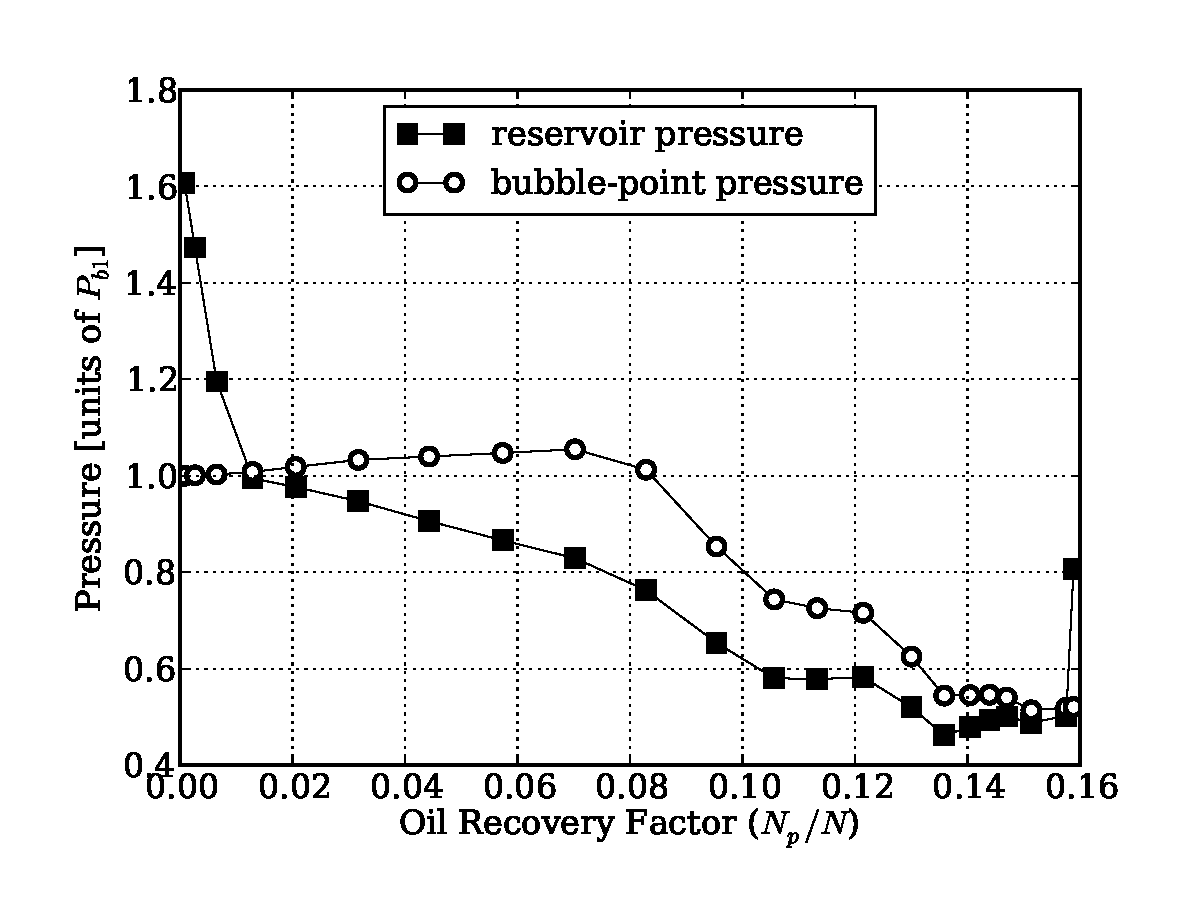
\includegraphics[width=\linewidth]{./python/matbal_p}
\caption{Reservoir pressure and bubble-point pressure as functions of recovery factor. Once depletion goes below bubble-point, pressure is hardly recovered for a saturated reservoir due to high system compressibility. Pressure is here given in units of the original bubble-point pressure.}
\label{fig: matbal_p}
\end{figure}

\begin{figure}
\centering
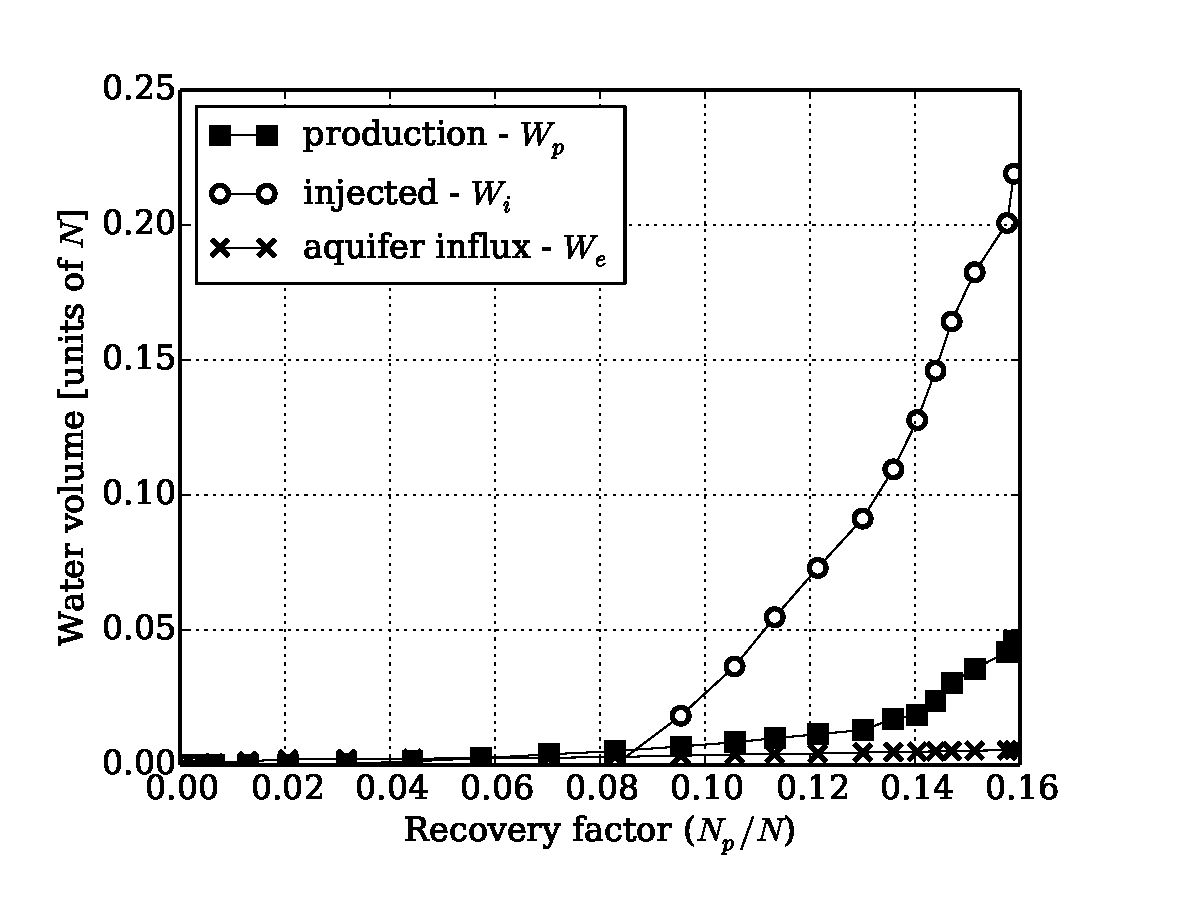
\includegraphics[width=\linewidth]{./python/matbal_water}
\caption{Volume of water production and injection and aquifer influx.}
\label{fig: matbal_water}
\end{figure}

\begin{figure}
\centering
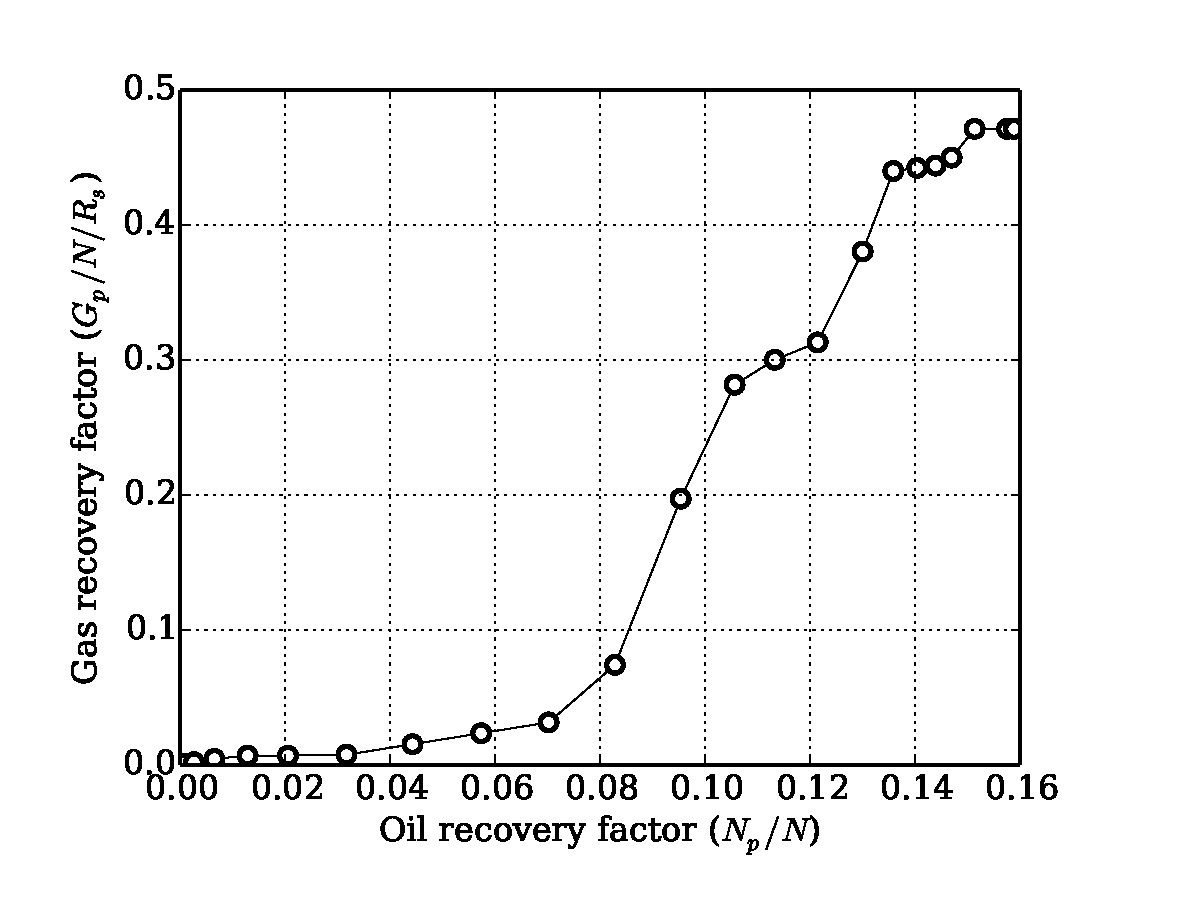
\includegraphics[width=\linewidth]{./python/matbal_gas}
\caption{Volume of gas production.}
\label{fig: matbal_gas}
\end{figure}

\begin{figure}
\centering
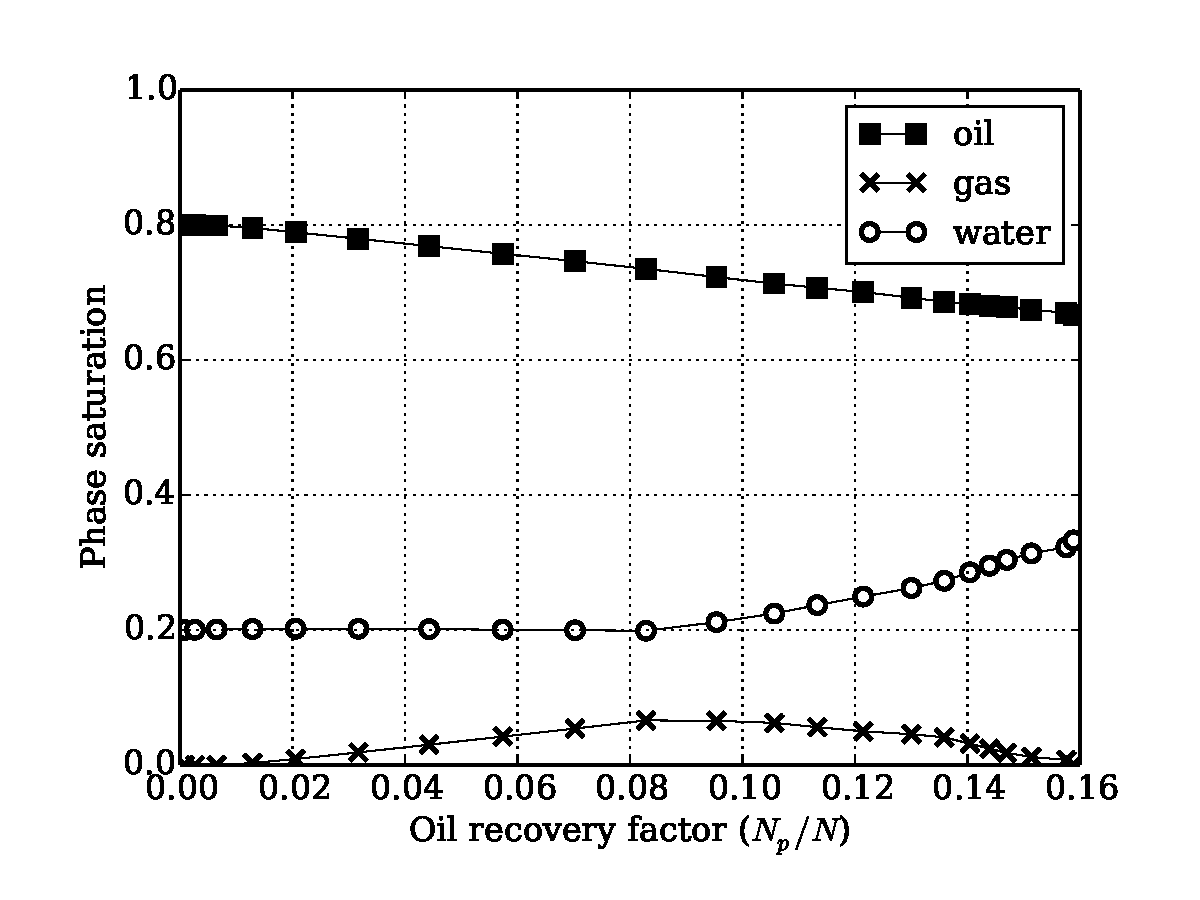
\includegraphics[width=\linewidth]{./python/matbal_S}
\caption{Phase saturations. Gas saturation is reduced as water injection progresses.}
\label{fig: matbal_s}
\end{figure}


\begin{figure}
\centering
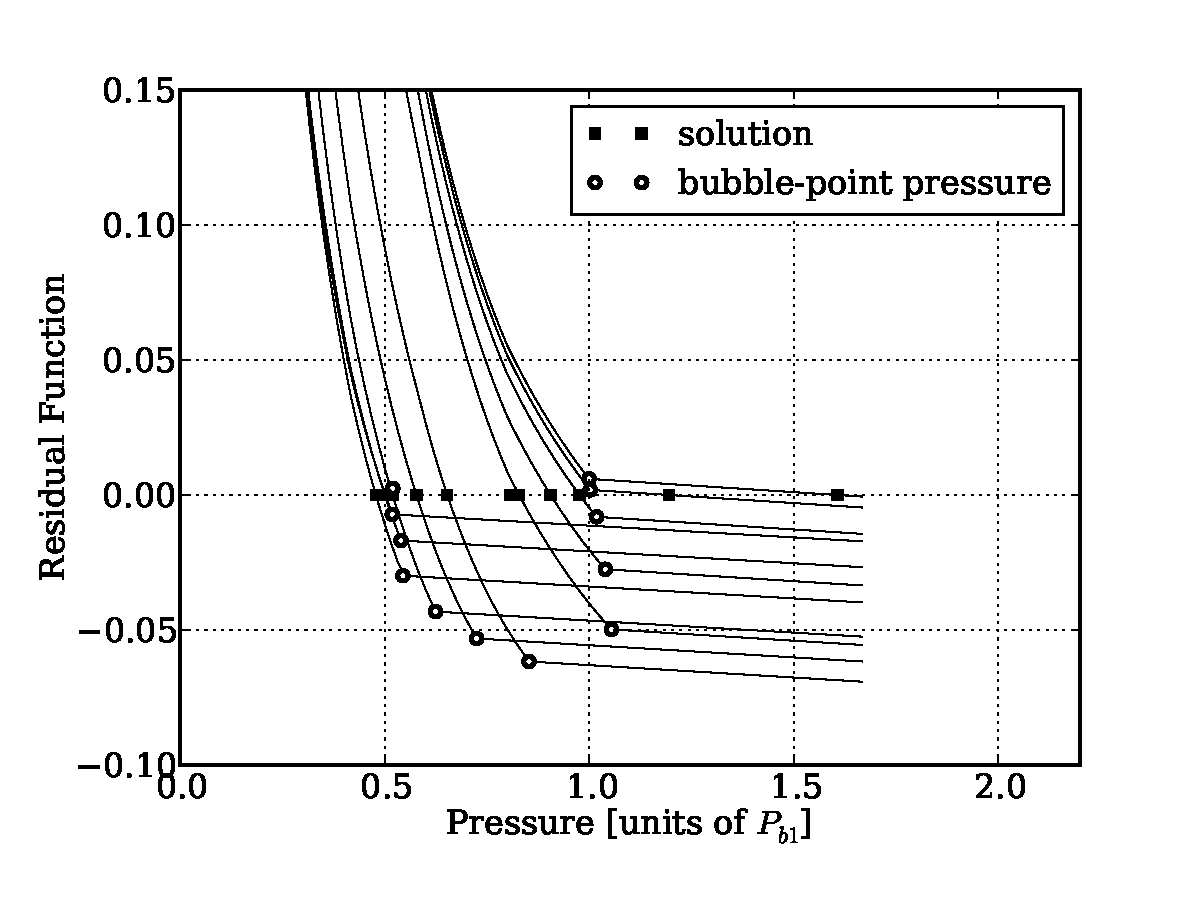
\includegraphics[width=\linewidth]{./python/matbal_res}
\caption{Shape of residual function ($\varepsilon$). Each curve corresponds to different volumes of production and injection. Residual function monotonically decreases with pressure and it has no derivative at the bubble-point.}
\label{fig: epsilon}
\end{figure}

\begin{figure}
\centering
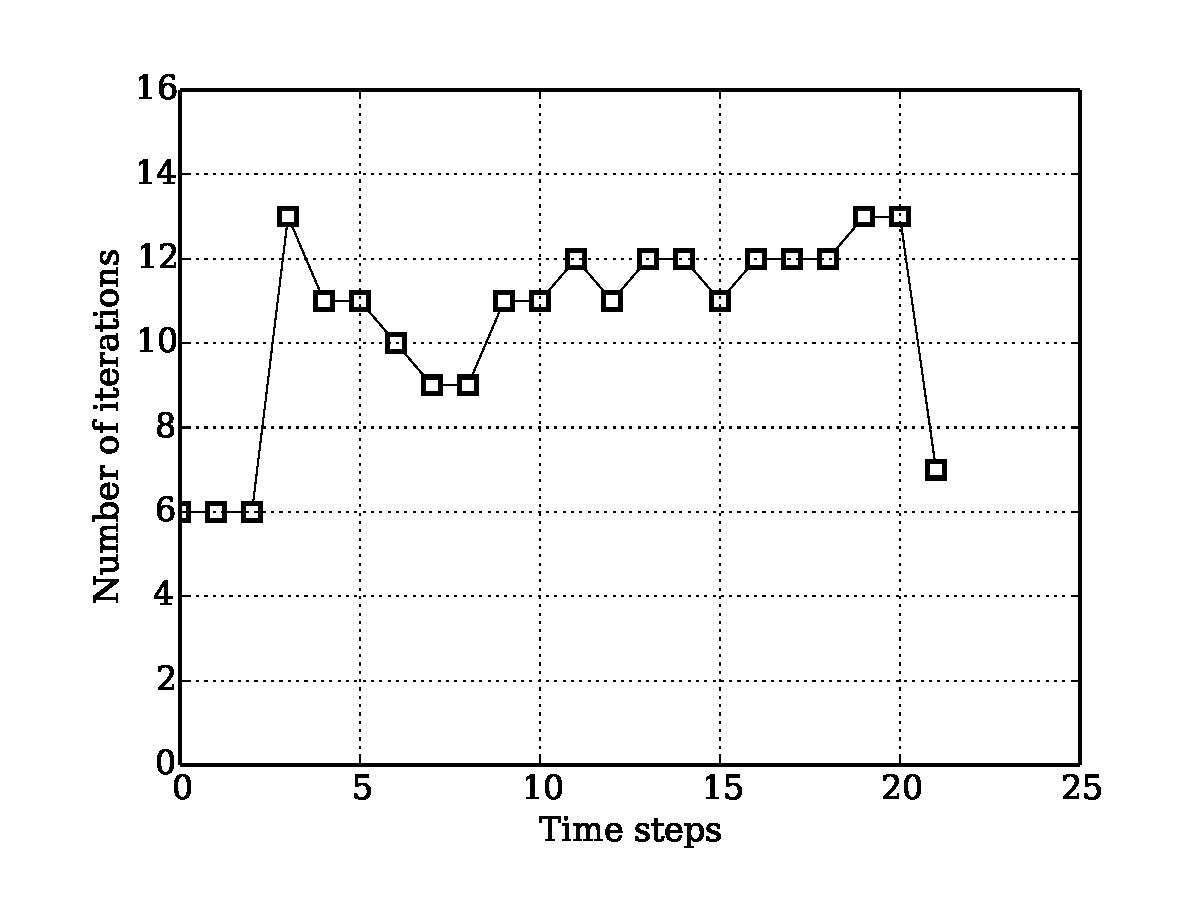
\includegraphics[width=\linewidth]{./python/matbal_iter}
\caption{Count of newtonian iterations required to compute pressure with accuracy within $0.001$ units of initial bubble-point presure.}
\label{fig: iter}
\end{figure}

\begin{figure}
\centering
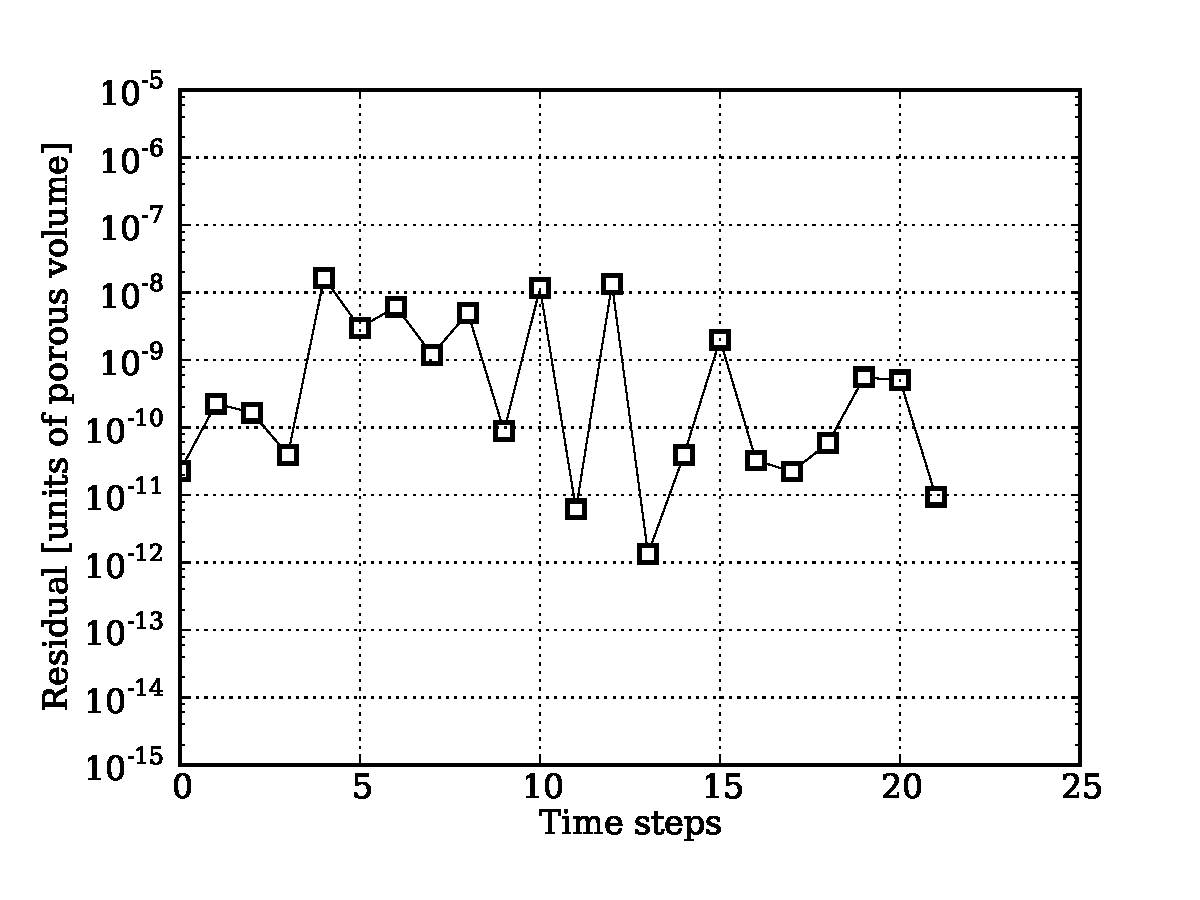
\includegraphics[width=\linewidth]{./python/matbal_residual}
\caption{Residual of numerical solution in units of porous volume.}
\label{fig: residual}
\end{figure}

\begin{table*}
\small
\centering
\begin{tabular}{ll}
\toprule
\multicolumn{2}{l}{\textit{Material Balance Equations}}\\
\midrule
oil & $S_{o2} = \left(N-N_p\right) B_{o2}/V_{p2}$ \label{eq: oiltab}
\\
water & $S_{w2} = \left(W+W_i+W_e-W_p\right) B_{w2}/V_{p2}$\\
gas & $S_{g2}=\left\lbrace N\left[\left(R_{s1}-R_{s2}\right)+m B_{o1}/B_{g1}\right]+N_p R_{s2}+G_i-G_p\right\rbrace Bg_2/V_{p2}$ \\
bubble-point pressure & $R_{s2}\left(P_b\right) = \left[N\left(m B_{1}/B_{g1} +R_{s1}\right)+G_i-G_p\right]/\left(N-N_p\right)$ \\
pressure & $F_p - F_i= N E_o + mN E_g + W E_w +C$ \\
\midrule
\multicolumn{2}{l}{\textit{Definition of terms in pressure equation}} \\
\midrule
fluid production & $F_p=N_p \left[B_{o2} + \left(G_p/N_p -R_{s2}\right)B_{g2}\right]+W_p B_{w2}$ \\
fluid injection and influx & $F_i=\left(W_i +W_e\right) B_{w2}+G_{i}B_{g2}$ \\
oil phase expansion & $E_o=\left(B_{o2}-B_{o1}\right) - \left(R_{so2}-R_{so1}\right)B_{g2}$ \\
gas phase expansion & $E_g = B_{o1}\left(B_{g2}/B_{g1}-1\right)$ \\
water volume expansion & $E_w = B_{w2}-B_{w1}$\\
porous volume contraction & $C=V_{p2}- V_{p1}$\\ \bottomrule
\end{tabular}
\caption{Complete set of material balance equations.}
\label{tab: MBE}
\end{table*}

% % %
% Calcular derivada da função resíduo com relação à pressão.
% % %

\end{document}